\section*{Avant Propos}

Afin d'analyser et classifier des images 2D ou imageries 3D, il est primordial d'être capable d'extraire de ces dernières un ensemble d'informations ou "\textit{features}" qui décrivent au mieux et nous renseigne sur la nature de celles-ci.\\
On pourrait citer par exemple des critères comme la taille de la boite englobante (en anglais : \textit{bounding box}), ou encore le volume de la forme pour une pièce mécanique en 3D, en passant par la surface de cette dernière. Le critères isopérimétrique (mesure de compacité) est un excellent exemple de facteur classifiant. Il permet de discriminer, avec une bonne précision, différentes pièces mécaniques à partir de modèles 3D [M. Bruneau et al]~\cite{Bruneau2014}.

Dans le cadre de ce stage,\\
\begin{itemize}
	\item	L'accent sera porté sur une analyse d'\textbf{images en 2D}.\\
	\item	Nous cherchons à rétro-concevoir de grands ensembles mécaniques, une attention à la gestion de \textbf{grands volumes de données} doit être apportée durant tout le déroulement du projet.\\
	\item	Mettre en place une \textbf{méthode d'extraction de descripteurs} d'un fichier image (en anglais : \textit{Feature Extractor}).\\
	\item	Cette \textbf{méthode} d'extraction doit être \textbf{automatisable}. Il n'est pas envisageable, dans le cadre de notre étude, de venir renseigner à la main chacun de ces descripteurs.	
\end{itemize}
\vspace{3mm}
  

\section{Les ShockGraphs}

\subsection{État de l'art et méthodes d'extraction de descripteurs.}

Suite à trois semaines d'analyse de la littérature scientifique, il en est ressorti plusieurs méthodes qui pourraient satisfaire nos besoins. La plupart de ces méthodes est directement dérivée du domaine de la \textbf{Vision par Ordinateur}.

J'ai testé plusieurs méthodes basées sur différentes approches du problèmes :
\begin{itemize}
	\item Filtre de Canny
	\item Algorithme SURF
	\item Réseaux de Convolutions
	\item ShockGraphs
	\item \ldots
\end{itemize}
\vspace{3mm}

\subsection{Étude de l'algorithme SURF.}

L'algorithme SURF~\cite{SURF} ou \textbf{S}peeded \textbf{U}p \textbf{R}obust \textbf{F}eatures a été présenté en 2006 et révisé en 2008 par des chercheurs de l'ETH Zurich et de la Katholieke Universiteit Leuven \url{http://www.vision.ee.ethz.ch/~surf/download_ac.html}

Pour résumer simplement son principe, il se base sur la détection de points d'intérêt et de descripteurs. Il peut être utilisé afin de réaliser de la détection d'objets ou de la reconstruction 3D. Il est en parti inspiré de l'algorithme SIFT~\cite{Lowe1999}, \textbf{S}cale-\textbf{I}nvariant \textbf{F}eature \textbf{T}ransform. Cependant SURF se veut plus robuste et rapide en pratique.

\begin{figure}[H]
    \centering
    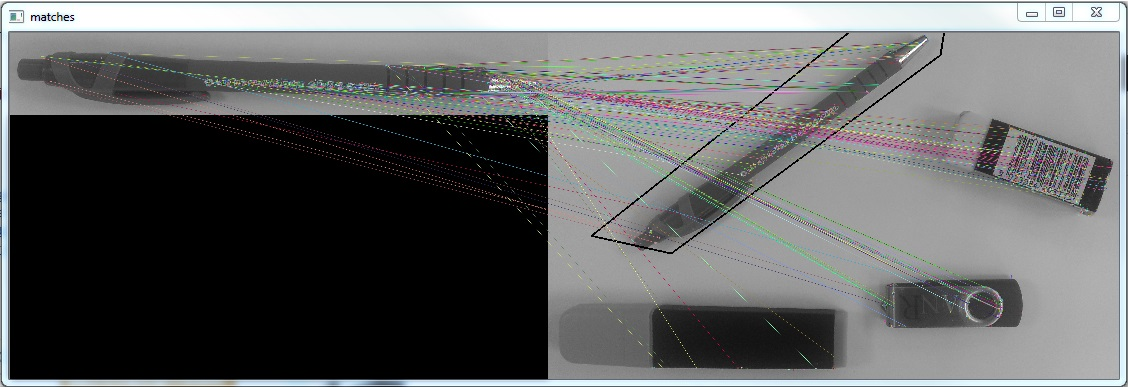
\includegraphics[height=5.5cm]{CannySurfClean.jpg}
	\caption{Output d'un test avec l'algorithme SURF, cible totalement visible} 
\end{figure}
\vspace{-6mm}

\begin{figure}[H]
    \centering
    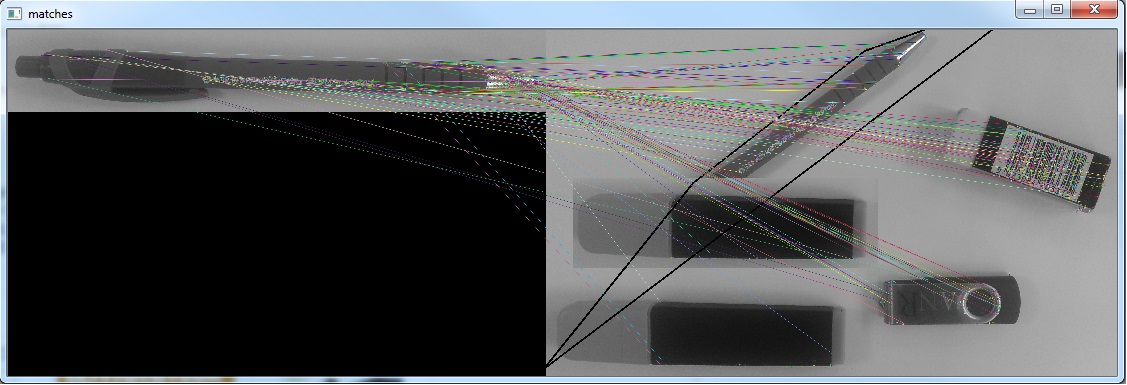
\includegraphics[height=5.5cm]{CannySurfPartiallyMasked.jpg}
	\caption{Output d'un test avec l'algorithme SURF, cible partiellement visible}\label{image.CannySurfPartiallyMasked} 
\end{figure}
\vspace{-6mm}

Il apparait que l'algorithme SURF manque de précision et vient \textit{accrocher} tous les objets de la scène. Une investigation plus poussée a permis de mettre en évidence que l'algorithme, étant basé sur la détection de points d'intérêt, n'est pas capable d'apprendre une \textbf{forme} mais uniquement les \textbf{détails} d'un objet spécifique. Raisons qui font de l'algorithme SURF un \textbf{mauvais candidat} pour notre étude.

\clearpage
\subsection{Tests préliminaires sur le fonctionnement des ShockGraphs}

Suite à mes recherches bibliographiques, j'ai pu mettre en évidence les travaux sur les ShockGraphs. Ce sont des graphs qui décrivent une forme binaire 2D (Blanche ou Noire, pas de gris) par le biais d'un \textit{squelette} ou \textit{axe médian de Blum}. Leur fonctionnement et leur utilisation est décrite par [K. Siddiqi et al]~\cite{Siddiqi1999}. Un démonstrateur scientifique ainsi qu'une méthode de comparaison de ces graphs a été mise au point par [D. Macrini et al]~\cite{Macrini2002} dans le cadre de son mémoire de Master.

À partir de ces travaux, j'ai pu mettre sur pied assez rapidement un test mettant en évidence la pertinence de la méthode relative à notre usage. Et je dois bien admettre avoir été bluffé par la précision de cette méthode. Sentiment qui semble avoir été partagé autour de moi.

J'ai donc créé, pour le test, un jeu de données d'entrainement et un jeu de test (ou validation). Chacun contenant un ensemble de vues des pièces mécaniques suivantes:
\begin{itemize}
	\item 	Piston
	\item	Bielle
	\item	Assemblage Piston/Bielle
	\item	Roue dentée
\end{itemize}
\vspace{5mm}

\begin{figure}[H]
    \centering
    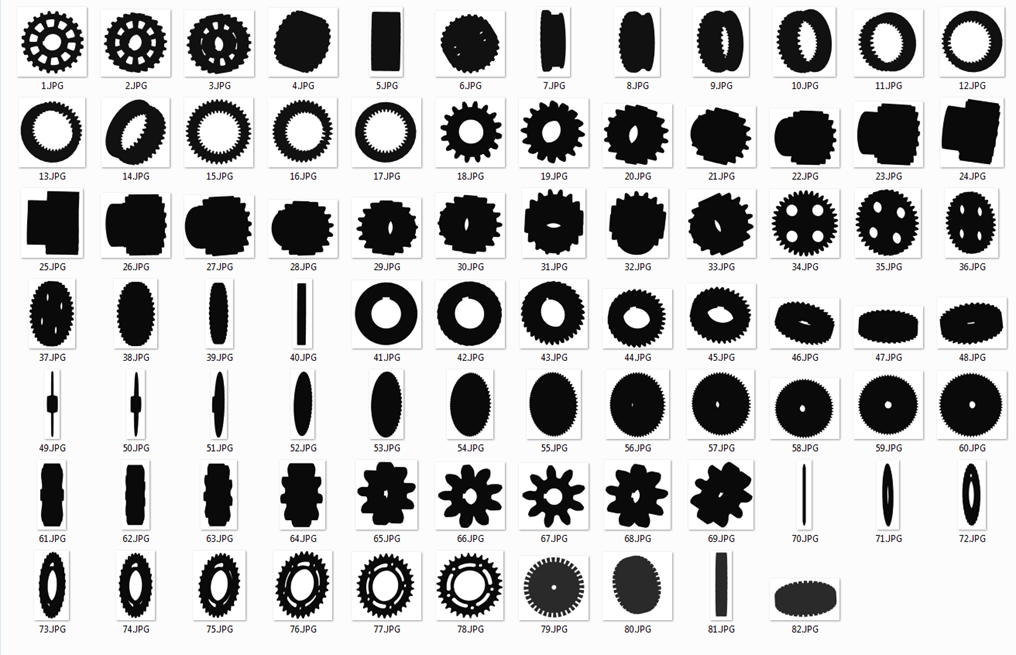
\includegraphics[height=7cm]{datasetShock.png}
	\caption{Exemple de base de connaissances sur les roues dentées, en vue du test des ShockGraphs}\label{image.ShockGearDataset} 
\end{figure}
\vspace{-4mm}

\begin{figure}[H]
    \centering
    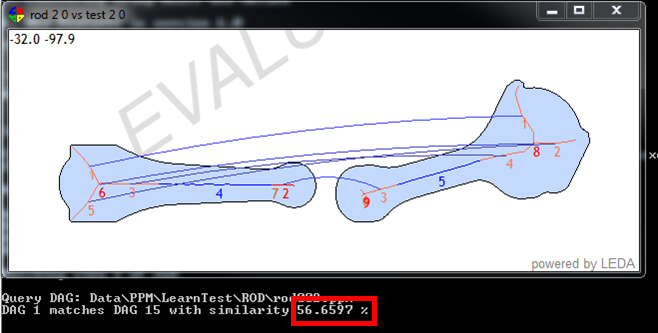
\includegraphics[height=5.5cm]{ShockTest1.png}
	\caption{Output d'un test utilisant les ShockGraphs, \textbf{56.6597\% de match}.}\label{image.ShockTest1} 
\end{figure}


\clearpage

\subsection{Principe de fonctionnement des ShockGraphs.}

\subsubsection{L'axe Médian de Blum}

L'axe médian de Blum est une méthode permettant de représenter la forme d'un objet en trouvant son squelette topologique.

On obtient ainsi un ensemble de \textbf{courbes connectées} entre elles. Pour information, la fonction \textit{bwmorph('skel')} dans Matlab permet de l'obtenir.

Cette méthode présente tout de même quelques problèmes :
\begin{itemize}
	\item De petits changements dans la forme peuvent avoir un fort impact sur le squelette final.
	\item La réaction est non prévisible en cas d'occlusion d'une partie de la forme.
\end{itemize}
\vspace{8mm}
\begin{figure}[H]
    \centering
    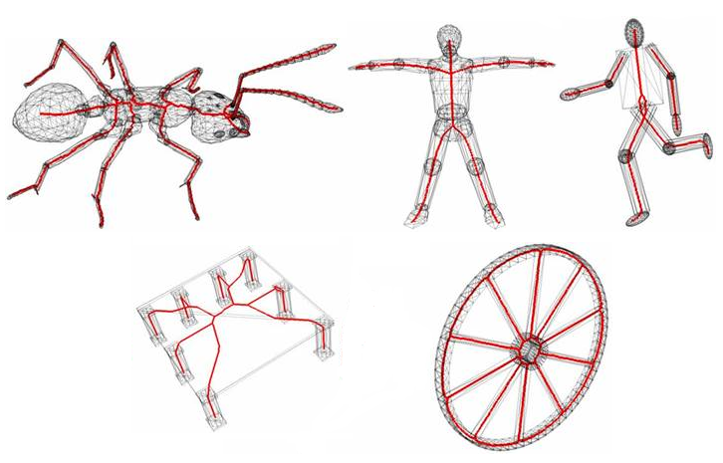
\includegraphics[height=10cm]{skelitization.png}
	\caption{Illustration du résultat d'un algorithme calculant \textbf{l'axe Median de Blum}.}\label{image.skel} 
\end{figure}

\subsubsection{La grammaire des ShockGraphs}


K. Siddiqi et al~\cite{Siddiqi1999} ont remarqué la forte ressemblance entre l'axe Median de Blum et la structure d'un graph. De plus ce squelette semble être tout à fait caractéristique d'une forme définie. Qui n'a d'ailleurs jamais schématiser un Homme à la manière présentée sur l'image ci-dessus ? 

Ils ont mis au point un processus pour générer un graph qu'ils ont appelé \textbf{ShockGraph} à partir de ces courbes connectées.

Afin d'obtenir le ShockGraph à partir des courbes connectées, on analyse la structure 2D de l'image et on en détermine le type de nœud. Quatres types différents sont possibles :

\begin{figure}[H]
    \centering
    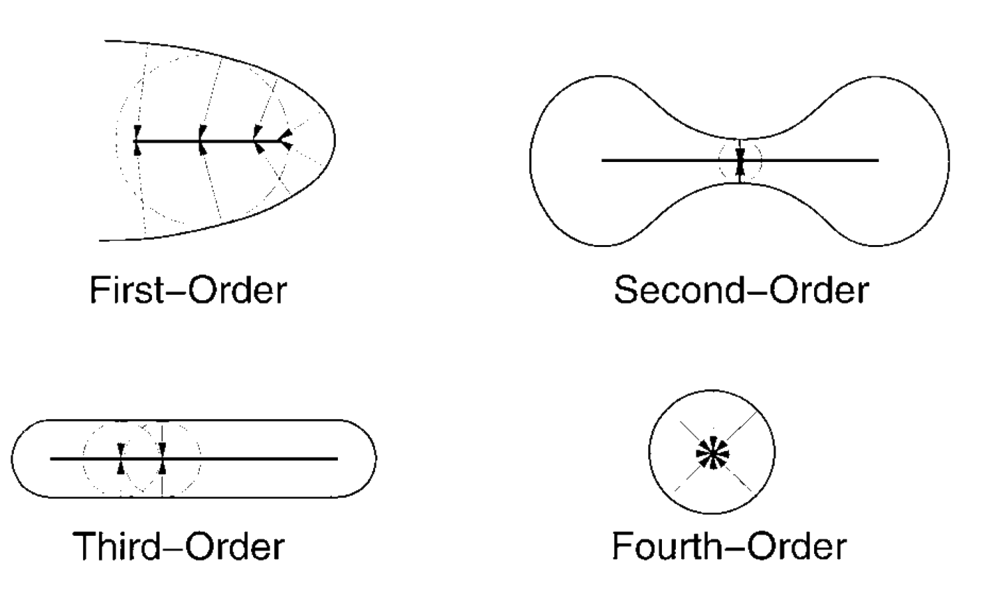
\includegraphics[height=10cm]{Node.png}
	\caption{4 Types de Noeuds existent afin de générer un ShockGraph.}\label{image.skel} 
\end{figure}

A cela, il convient de rajouter la grammaire suivante afin d'établir la position des nœuds entre eux et leurs connections. A savoir le ShockGraph est un graph \textbf{direct et acyclique}.\\


\begin{itemize}
	\item \textbf{Vertices} : V = \{1,..., n\} \\
	
	\item \textbf{Edges} (i, j) ∈ E ⊆ V × V \\
	Dirigée de i => j, si et seulement si i ≠ j , i \& j sont connectés dans le squelette.\\
	
	\item \textbf{Labels} $\gamma$ : V → l, avec l ∈ \{1, 2, 3, 4, n-2, \#, $\Phi$\}\\
	Avec: \#: Start Symbol \&\& $\Phi$ : Terminal Symbol.\\
	
	\item \textbf{Topology} : ∀ j ∈ V avec $\gamma$ (j) ≠ \#, ∃i ∈ V avec (i, j) ∈ E : Si j n’est pas racine alors il a au moins un antécédant.

\end{itemize}

\clearpage